%%%%%%%%%%%%%%%%%%%%%%%%%%%%%%%%%%%%%%%%%
% a0poster Landscape Poster
% LaTeX Template
% Version 1.0 (22/06/13)
%
% The a0poster class was created by:
% Gerlinde Kettl and Matthias Weiser (tex@kettl.de)
%
% This template has been downloaded from:
% http://www.LaTeXTemplates.com
%
% License:
% CC BY-NC-SA 3.0 (http://creativecommons.org/licenses/by-nc-sa/3.0/)
%
%%%%%%%%%%%%%%%%%%%%%%%%%%%%%%%%%%%%%%%%%

%-------------------------------------------------------------------------------
%	PACKAGES AND OTHER DOCUMENT CONFIGURATIONS
%-------------------------------------------------------------------------------

\documentclass[a0, landscape]{a0poster}

\usepackage{multicol} % This is so we can have multiple columns of text side-by-side
\columnsep=100pt % This is the amount of white space between the columns in the poster
\columnseprule=3pt % This is the thickness of the black line between the columns in the poster

\usepackage[svgnames]{xcolor} % Specify colors by their 'svgnames', for a full list of all colors available see here: http://www.latextemplates.com/svgnames-colors

%\usepackage{times} % Use the times font
% \usepackage{palatino} % Uncomment to use the Palatino font
\usepackage{fontspec}
\setmainfont{Latin Modern Sans}

\usepackage{graphicx} % Required for including images
\graphicspath{{figures/}} % Location of the graphics files
\usepackage{booktabs} % Top and bottom rules for table
\usepackage[font=small,labelfont=bf]{caption} % Required for specifying captions to tables and figures
\usepackage{amsfonts, amsmath, amsthm, amssymb} % For math fonts, symbols and environments
\usepackage{wrapfig} % Allows wrapping text around tables and figures

\usepackage{listings}
\usepackage{color}

\definecolor{dkgreen}{rgb}{0,0.6,0}
\definecolor{gray}{rgb}{0.5,0.5,0.5}
\definecolor{mauve}{rgb}{0.58,0,0.82}

\lstset{
  %frame=tb,
  language=Python,
  aboveskip=2mm,
  belowskip=0mm,
  showstringspaces=false,
  columns=flexible,
  basicstyle={\small\ttfamily},
  numbers=none,
  numberstyle=\tiny\color{gray},
  keywordstyle=\color{blue},
  commentstyle=\color{dkgreen},
  stringstyle=\color{mauve},
  breaklines=true,
  breakatwhitespace=true,
  tabsize=3,
  framexleftmargin=15pt
  }


\begin{document}

%----------------------------------------------------------------------------------------
%	POSTER HEADER
%----------------------------------------------------------------------------------------

% The header is divided into three boxes:
% The first is 55% wide and houses the title, subtitle, names and university/organization
% The second is 25% wide and houses contact information
% The third is 19% wide and houses a logo for your university/organization or a photo of you
% The widths of these boxes can be easily edited to accommodate your content as you see fit

\begin{minipage}[b]{0.85\linewidth}
\veryHuge \color{NavyBlue} \textbf{Evaluating the accuracy of diffusion MRI models in the Human Connectome Project at scale with DIPY and Cloudknot} \color{Black}\\ % Title
%\Huge\textit{An Exploration of Complexity}\\[1cm] % Subtitle
\huge \textbf{Ariel Rokem\textsuperscript{1}, \& Adam Richie-Halford \textsuperscript{2}}\\ % Author(s)
\Large 1. The eScience Institute, 2. Dept. of Physics, Univ. of Washington \\ % University/organization
\Large Contact: \texttt{arokem@uw.edu} $|$ Download: \texttt{http://arokem.org/presentations/brainpi-dipy-2019}
\end{minipage}
%
%\begin{minipage}[b]{0.25\linewidth}
%\color{DarkSlateGray}\Large \textbf{Contact Information:}\\
%Department Name\\ % Address
%University Name\\
%123 Broadway, State, Country\\\\
%Phone: +1 (000) 111 1111\\ % Phone number
%Email: \texttt{john@LaTeXTemplates.com}\\ % Email address
%\end{minipage}
%
\begin{minipage}[b]{0.19\linewidth}

\includegraphics[width=10cm]{UWlogo.png}
\end{minipage}

\vspace{0.5cm} % A bit of extra whitespace between the header and poster content

%----------------------------------------------------------------------------------------

\begin{multicols}{3} % This is how many columns your poster will be broken into, a poster with many figures may benefit from less columns whereas a text-heavy poster benefits from more

%----------------------------------------------------------------------------%	Introduction
%----------------------------------------------------------------------------

\section*{Introduction}

\subsection*{The Human Connectome Project}

Diffusion MRI (dMRI) measurements provide detailed information about human brain
connectivity and microstructure \emph{in vivo}. HCP has measured high-quality
multi-modal MRI data from 1,200 individuals and is making these data publcly
available \cite{glasser2016}. Data can be accessed through Amazon's Simple
Storage Web Service (S3).

\subsection*{DIPY: Software framework for analysis of dMRI \cite{Garyfallidis2014FrontNeuroinf}}

\begin{minipage}[b]{1\linewidth}
\begin{minipage}[b]{0.35\linewidth}
    \begin{itemize}
    \item Open-source
    \item Community-developed
    \item Supported by NIBIB through the CRCNS program
    \end{itemize}
\end{minipage}
\begin{minipage}[b]{0.65\linewidth}
    
\includegraphics[height=3.5cm]{dipy-logo.png}
\end{minipage}
\end{minipage}

\subsection*{What model should we use to explain the data?}

open-source software library (\texttt{http://dipy.org/}) . 5-fold cross-validation was implemented using DIPY's cross-validation module \cite{Rokem2015PLoS}


\subsection*{Diffusion Tensor Imaging (DTI): 6 parameters}

Approximates diffusion in every voxel as a Gaussian distribution
\cite{Basser1994-hg}:

\vspace{2mm}
\begin{center}
\begin{large}

$S(\theta, b) = S_0 e^{\theta^T \mathbf{Q} \theta} $

\end{large}
\end{center}

\noindent $b$ is the \textbf {b-value},

\noindent $S_0$ is the signal in the absence of diffusion gradient sensitization ($b=0$)

\noindent $\mathbf{Q}$ is a positive-definite quadratic form:

\vspace{2mm}
\begin{center}

$\mathbf{D} = \begin{pmatrix} \sigma_{xx} & \sigma_{xy} & \sigma_{xz} \\
                              \sigma_{yx} & \sigma_{yy} & \sigma_{yz} \\
				                      \sigma_{zx} & \sigma_{zy} & \sigma_{zz} \\
\end{pmatrix} $

\end{center}

\subsection*{Diffusion Kurtosis imaging (DKI): 21 parameters}

DKI is an extension of DTI that accounts for non-Gaussian behavior in complex tissue, with many barriers to the diffusion process (cell membranes,
myelin sheaths, etc.) \cite{Jensen2005-vr}:

\vspace{2mm}
\begin{center}
\begin{large}

$ S(\theta, b)=S_{0}e^{-bD(\theta)+\frac{1}{6}b^{2}D(\theta)^{2}K(\theta)}$

\vspace{2mm}
\end{large}
\end{center}

\vspace{2mm}
\begin{center}
\begin{large}

$D(\theta)=\sum_{i=1}^{3}\sum_{j=1}^{3}\theta_{i}\theta_{j}Q_{ij}$

\vspace{2mm}
\end{large}
\end{center}

\vspace{2mm}
\begin{center}
\begin{large}

$K(\theta)=\frac{MD^{2}}{D(\theta)^{2}}\sum_{i=1}^{3}\sum_{j=1}^{3}\sum_{k=1}^{3} \sum_{l=1}^{3}\theta_{i}\theta_{j}\theta_{k}\theta_{l}W_{ijkl}$

\vspace{2mm}
\end{large}
\end{center}

$\mathbf{W}$ is a rank 4 tensor (3-by-3-by-3-by-3 matrix).

\vspace{-2mm}
\subsection*{Diffusion Statistics}

\begin{itemize}

\item Mean diffusivity (\textbf{MD}) characterizes the mean displacement of
water molecules within a voxel.

\item Fractional anisotropy (\textbf{FA}) characterizes the variance in
diffusivity in different directions.

\end{itemize}

\large

\noindent \textbf{Brain measurements that provide a close tie between brain tissue properties and behavior}.

\vfill
\columnbreak
\color{Navy}

\section*{Comparing models}

Cross-validation provides a flexible approach to comparing different models \cite{Rokem2015PLoS}

{\bf Problem: } Cross-validation is compute intense, so would take prohibitively long time if executed serially.

{\bf Solution: } Parallelize across subjects on AWS cloud computing.


%----------------------------------------------------------------------------%	RESULTS
%----------------------------------------------------------------------------

\section*{Cloud computing}

Cloud computing provides access to data and compute resources in a manner that is:

\begin{itemize}
\item{{\bf Scalable}. Massive compute resources can be deployed.}
\item{{\bf Elastic}. Resources can be provisioned and de-provisioned rapidly.}
\item{{\bf Robust}. Can handle large datasets and workloads.}
\item{{\bf Up to date}. The underlying compute technologies are updated by the cloud provider.}
\end{itemize}

\subsection*{But it is also:}

\begin{itemize}
\item{{\bf Challenging to learn.} Researchers using the cloud need to learn new terminology.}
\item{{\bf Hard to automate.} Complex APIs vs. clicking through web consoles.}
\item{{\bf Provisioning resources has overhead.} Especially in the absence of automation.}
\item{{\bf Not (yet?) a perfect match to scientific use-cases.} The major business case is developers building web-based platforms.}
\end{itemize}

\subsection*{Cloudknot}

A Python library that automates submission of scientific computing functions
to the Amazon Web Services Batch service \cite{adam_richie-halford-proc-scipy-2018}.

\texttt{https://richford.github.io/cloudknot/}

\begin{minipage}[b]{1\linewidth}
\begin{minipage}[b]{0.45\linewidth}
  
\includegraphics[height=3.5cm]{AWS.png}\\
  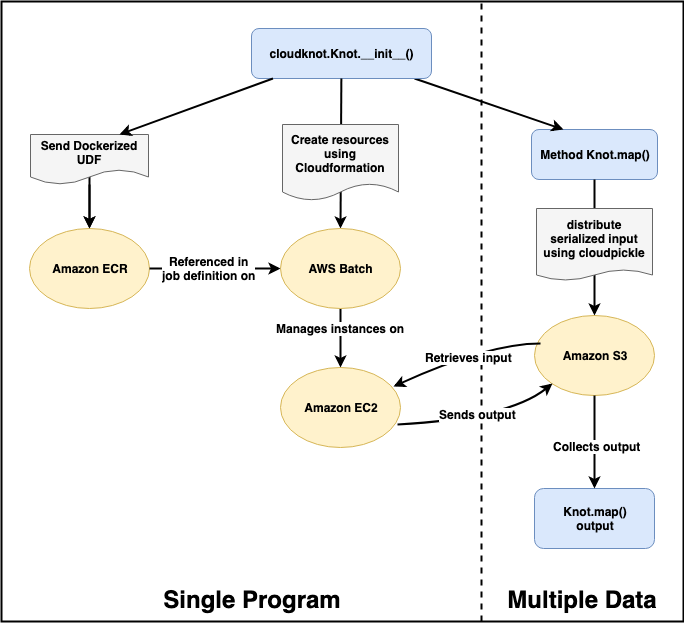
\includegraphics[width=14cm]{ck-architecture.png}
\end{minipage}
\begin{minipage}[b]{0.55\linewidth}
\begin{lstlisting}
import cloudknot as ck

def xval_hcp(subject):
	from dipy.reconst import dti
    import dipy.reconst.cross_validation as xval
	data = load_data(subject) # Loads data from S3
	model = dti.TensorModel(data['gradients'])
    pred = xval.kfold_xval(model, data, 5)
    cod = xval.coeff_of_determination(pred, data)
    upload_data(cod) # Save back into S3

# Creates the Docker image:
knot = ck.Knot(func=xval_hcp)
# Dispatches execution to AWS:
knot.map(['SUB1', ..., 'SUB100'])
\end{lstlisting}
\end{minipage}
\end{minipage}

\columnbreak

\section*{Results}

\noindent \textbf{We compared DKI and DTI using \emph{K-fold cross-validation}}

\subsection*{Model accuracy}
\normalsize

\noindent Cross-validated $R^2$: \textbf{A} Comparison of the full distribution
in a single subject, and comparison of the median (dashed line) in all subjects
for DKI (all b-values) and DTI (\textbf{B} all b-values, \textbf{C} only b=1,000
$s/mm^2$)  \hfill \break

\begin{minipage}[b]{1\linewidth}
  \large
  \begin{minipage}[b]{0.25\linewidth}
  \textbf{A}\\
  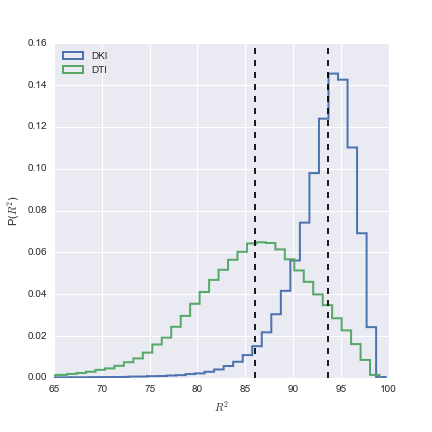
\includegraphics[width=11.5cm]{histogram_cod_dki_dti.png}
  \end{minipage}
\hfill
  \begin{minipage}[b]{0.25\linewidth}
  \textbf{B}\\
  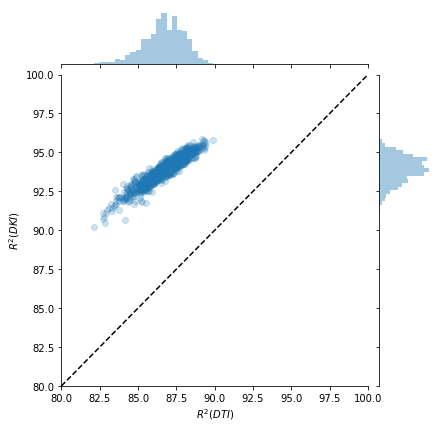
\includegraphics[width=12cm]{cod_dti_dki.png}
  \end{minipage}
\hfill
  \begin{minipage}[b]{0.25\linewidth}
  \textbf{C}\\
  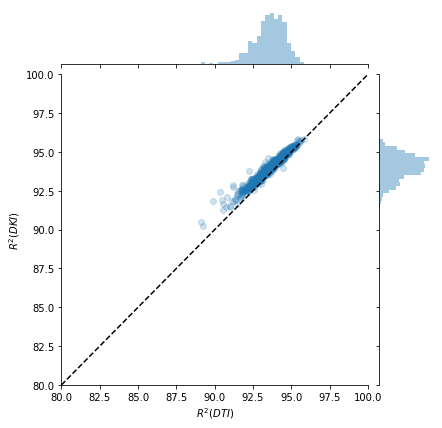
\includegraphics[width=12cm]{dti_1000_dki.png}
  \end{minipage}
\end{minipage}

%----------------------------------------------------------------------------
%	MATERIALS AND METHODS
%----------------------------------------------------------------------------

\color{SaddleBrown} % SaddleBrown color for the conclusions to make them stand out

\section*{Conclusions}
\large
\begin{itemize}

\item DKI more accurately fits the HCP data than DTI

\item DKI has the additional benefit that it provides additional parameters that
lend themselves to a richer biophysical interpretation of the signal.

\item Open-source software for analysis of human white matter scales on cloud computing.
\end{itemize}

\color{DarkSlateGray} % Set the color back to DarkSlateGray for the rest of the content

%---------------------------------------------------------------------------	REFERENCES
%----------------------------------------------------------------------------

\nocite{*} % Print all references regardless of whether they were cited in the poster or not
\bibliographystyle{plain} % Plain referencing style
\footnotesize \bibliography{poster} % Use the example bibliography file sample.bib

%----------------------------------------------------------------------------%	ACKNOWLEDGEMENTS
%----------------------------------------------------------------------------
\subsection*{Acknowledgements} \footnotesize



\includegraphics[height=2.6cm]{NIBIB.png}\\

\includegraphics[height=2.6cm]{SloanLogo.png}

\includegraphics[height=2.6cm]{MooreFdn.png}

\includegraphics[height=2.6cm]{eSciencelogo.png}
%----------------------------------------------------------------------------

\end{multicols}
\end{document}
